
\section{Descrição do sistema}
\subsection{Temporização dos semáforos}

\setlength{\parindent}{2cm}
São definidos três temporizações para o sistema de semáforos. Na temporização A, os semáforos possuem tempos equivalentes. Na temporização B, o semáforo correspondente à avenida Açaí possui um tempo mais elevado. Ainda há um terceiro modo no qual os semáforos devem estar piscando a luz amarela, informando que o sistema está desativado. 

\vskip3ex
\begin{figure}
\centering
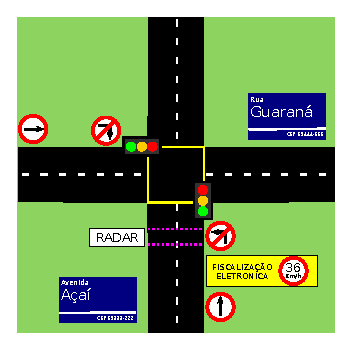
\includegraphics[width=0.99\columnwidth]{Semaforo.eps}
\end{figure}
\vskip3ex

Os tempos de luz verde de cada semáforo em relação à temporização desejada estão descritos na Table~\ref{tab01}.

\begin{table}[]
\caption{Semáforo Parnamirim-Natal}
\label{tab01}
\begin{tabular}{c | c | c | c}
\hline
Semáforo & A   & B   & C   \\ \hline
Av. Açaí    & 20s & 30s  & - \\ 
R. Guaraná  & 20s  & 10s  & -  \\ \hline
\end{tabular}
\end{table}
\vskip2ex

O tempo de luz amarela deve ser de 3 segundos.

\subsection{Radar de velocidade}

\setlength{\parindent}{2cm}
O radar de velocidade é composto por dois sensores de pressão localizados na via e que estão distantes 30 metros um do outro. O cálculo da velocidade do veículo é baseado no intervalo de tempo entre as ativações dos dois sensores. Se a velocidade do veículo for superior a 36 quilômetros por hora, o motorista deverá ser processado.

\section{Implementação}

O aluno deverá implementar o sistema de semáforos em FPGA, utilizando os seguintes pinos:
\begin{itemize}
    \justifying
    \item LEDR[0], LEDR[1] e LEDR[2] - Luzes vermelha, amarela e verde do semáforo da Av. Açaí respectivamente.
    \item LEDG[6], LEDG[7] e LEDG[8] - Luzes vermelha, amarela e verde do semáforo da R. Guaraná respectivamente.
    \item SW[0] e SW[1] - Chaves que selecionam os modos: "00" para temporização A, "01" para temporização B e "10" para temporização C.
    \item KEY[0] e KEY[1] -  Sensores de pressão (ativados no '0').
    \item LEDG[0] - Aviso de veículo com velocidade adequada.
    \item LEDR[17] - Aviso de veículo com velocidade inadequada.
\end{itemize}

\section{Apresentação de Resultados}
Toda a implementação do projeto utilizará apenas os conceitos apresentados em sala de aula, tendo uma pontuação reduzida significativamente caso isso seja violado.

Os resultados deverão ser apresentados em formato de pôster como este disponível em: \href{www.github.com/~kenreurison/posterModelo}{Pôster Modelo}. Contendo:
\begin{itemize}
    \item Descrição da metodologia;
    \item Diagramas \textit{RTL}, com comentários;
    \item Simulações \textit{waveform} que descrevem o funcionamento dos semáforos e do radar.
\end{itemize}

O prazo para a entrega do pôster com os códigos fontes do projeto compactados será \textbf{01 de Novembro} (não precisam imprimir) com apresentação do grupo no dia \textbf{02 de Novembro}.
